\chapter{閉曲線の曲率とトポロジーの関係}

今までは$\mathbb{R}^3$に埋め込まれた曲線を扱ってきましたが、平面$\mathbb{R}^2$に埋め込まれた曲線は扱いやすいため、より豊かな結果があります。
特に平面曲線$\gamma:[a,b]\to\mathbb{R}^2$であって、$\gamma(a)=\gamma(b)$を満たすもの、すなわち\textbf{閉曲線}の曲率から、今までの微分と積分とによる幾何学と代数トポロジーとの接点が現れてきます。

\section{閉曲線の定義}

まず一応、平面曲線の定義を行います。
\begin{definition}[平面曲線]
  $(\gamma,I)$が\textbf{平面曲線}であるとは、$I\subset\mathbb{R}$は閉区間であり、$\gamma:I\to\mathbb{R}^2$は$C^2$級写像であるときをいう。
\end{definition}

\begin{definition}[閉曲線]
  平面曲線$(\gamma,[a,b])$が\textbf{閉曲線}であるとは、$\gamma(a)=\gamma(b)$かつ、
  \[
    \left.\frac{d\gamma(t)}{dt}\right|_{t=a}=\left.\frac{d\gamma(t)}{dt}\right|_{t=b}
  \]
  を満たす時を言う。
\end{definition}
微分に関する条件は、曲線の始点と終点が滑らかに繋がっているようにするために仮定しています。

\subsection{閉曲線の例}

もちろん、円は閉曲線です。
\begin{example}
  \[
    \gamma:[0,2\pi]\to\mathbb{R}^2;t\mapsto(\cos(t),\sin(t))
  \]
  は閉曲線である。
\end{example}

一般に、楕円
\[
  \gamma:[0,2\pi]\to\mathbb{R}^2;t\mapsto(a\cos(t),b\sin(t))
\]
も閉曲線です。

\begin{example}[リサージュ曲線]\label{example:Lissajous_curve}
  $m,n\in\mathbb{Z}\setminus\{0\}$を互いに素な整数であり、片方は偶数であるとする。
  このとき、
  \[
    \gamma:[0,2\pi]\to\mathbb{R}^2;t\mapsto(\sin(mt),\sin(nt))
  \]
  は閉曲線である。
\end{example}
\begin{proof}
  $\gamma(0)=\gamma(2\pi)$は明らか。
  また、
  \[
    \frac{d\gamma(t)}{dt}=(m\cos(mt),n\cos(nt))
  \]
  ゆえ、$d\gamma(t)/dt|_{t=0}=d\gamma(t)/dt|_{t=2\pi}=(m,n)$も成り立つ。
\end{proof}
この曲線は\textbf{リサージュ曲線}と呼ばれる有名な曲線の一種です。
こんな感じの曲線になります。
\begin{figure}[htbp]
  \centering
  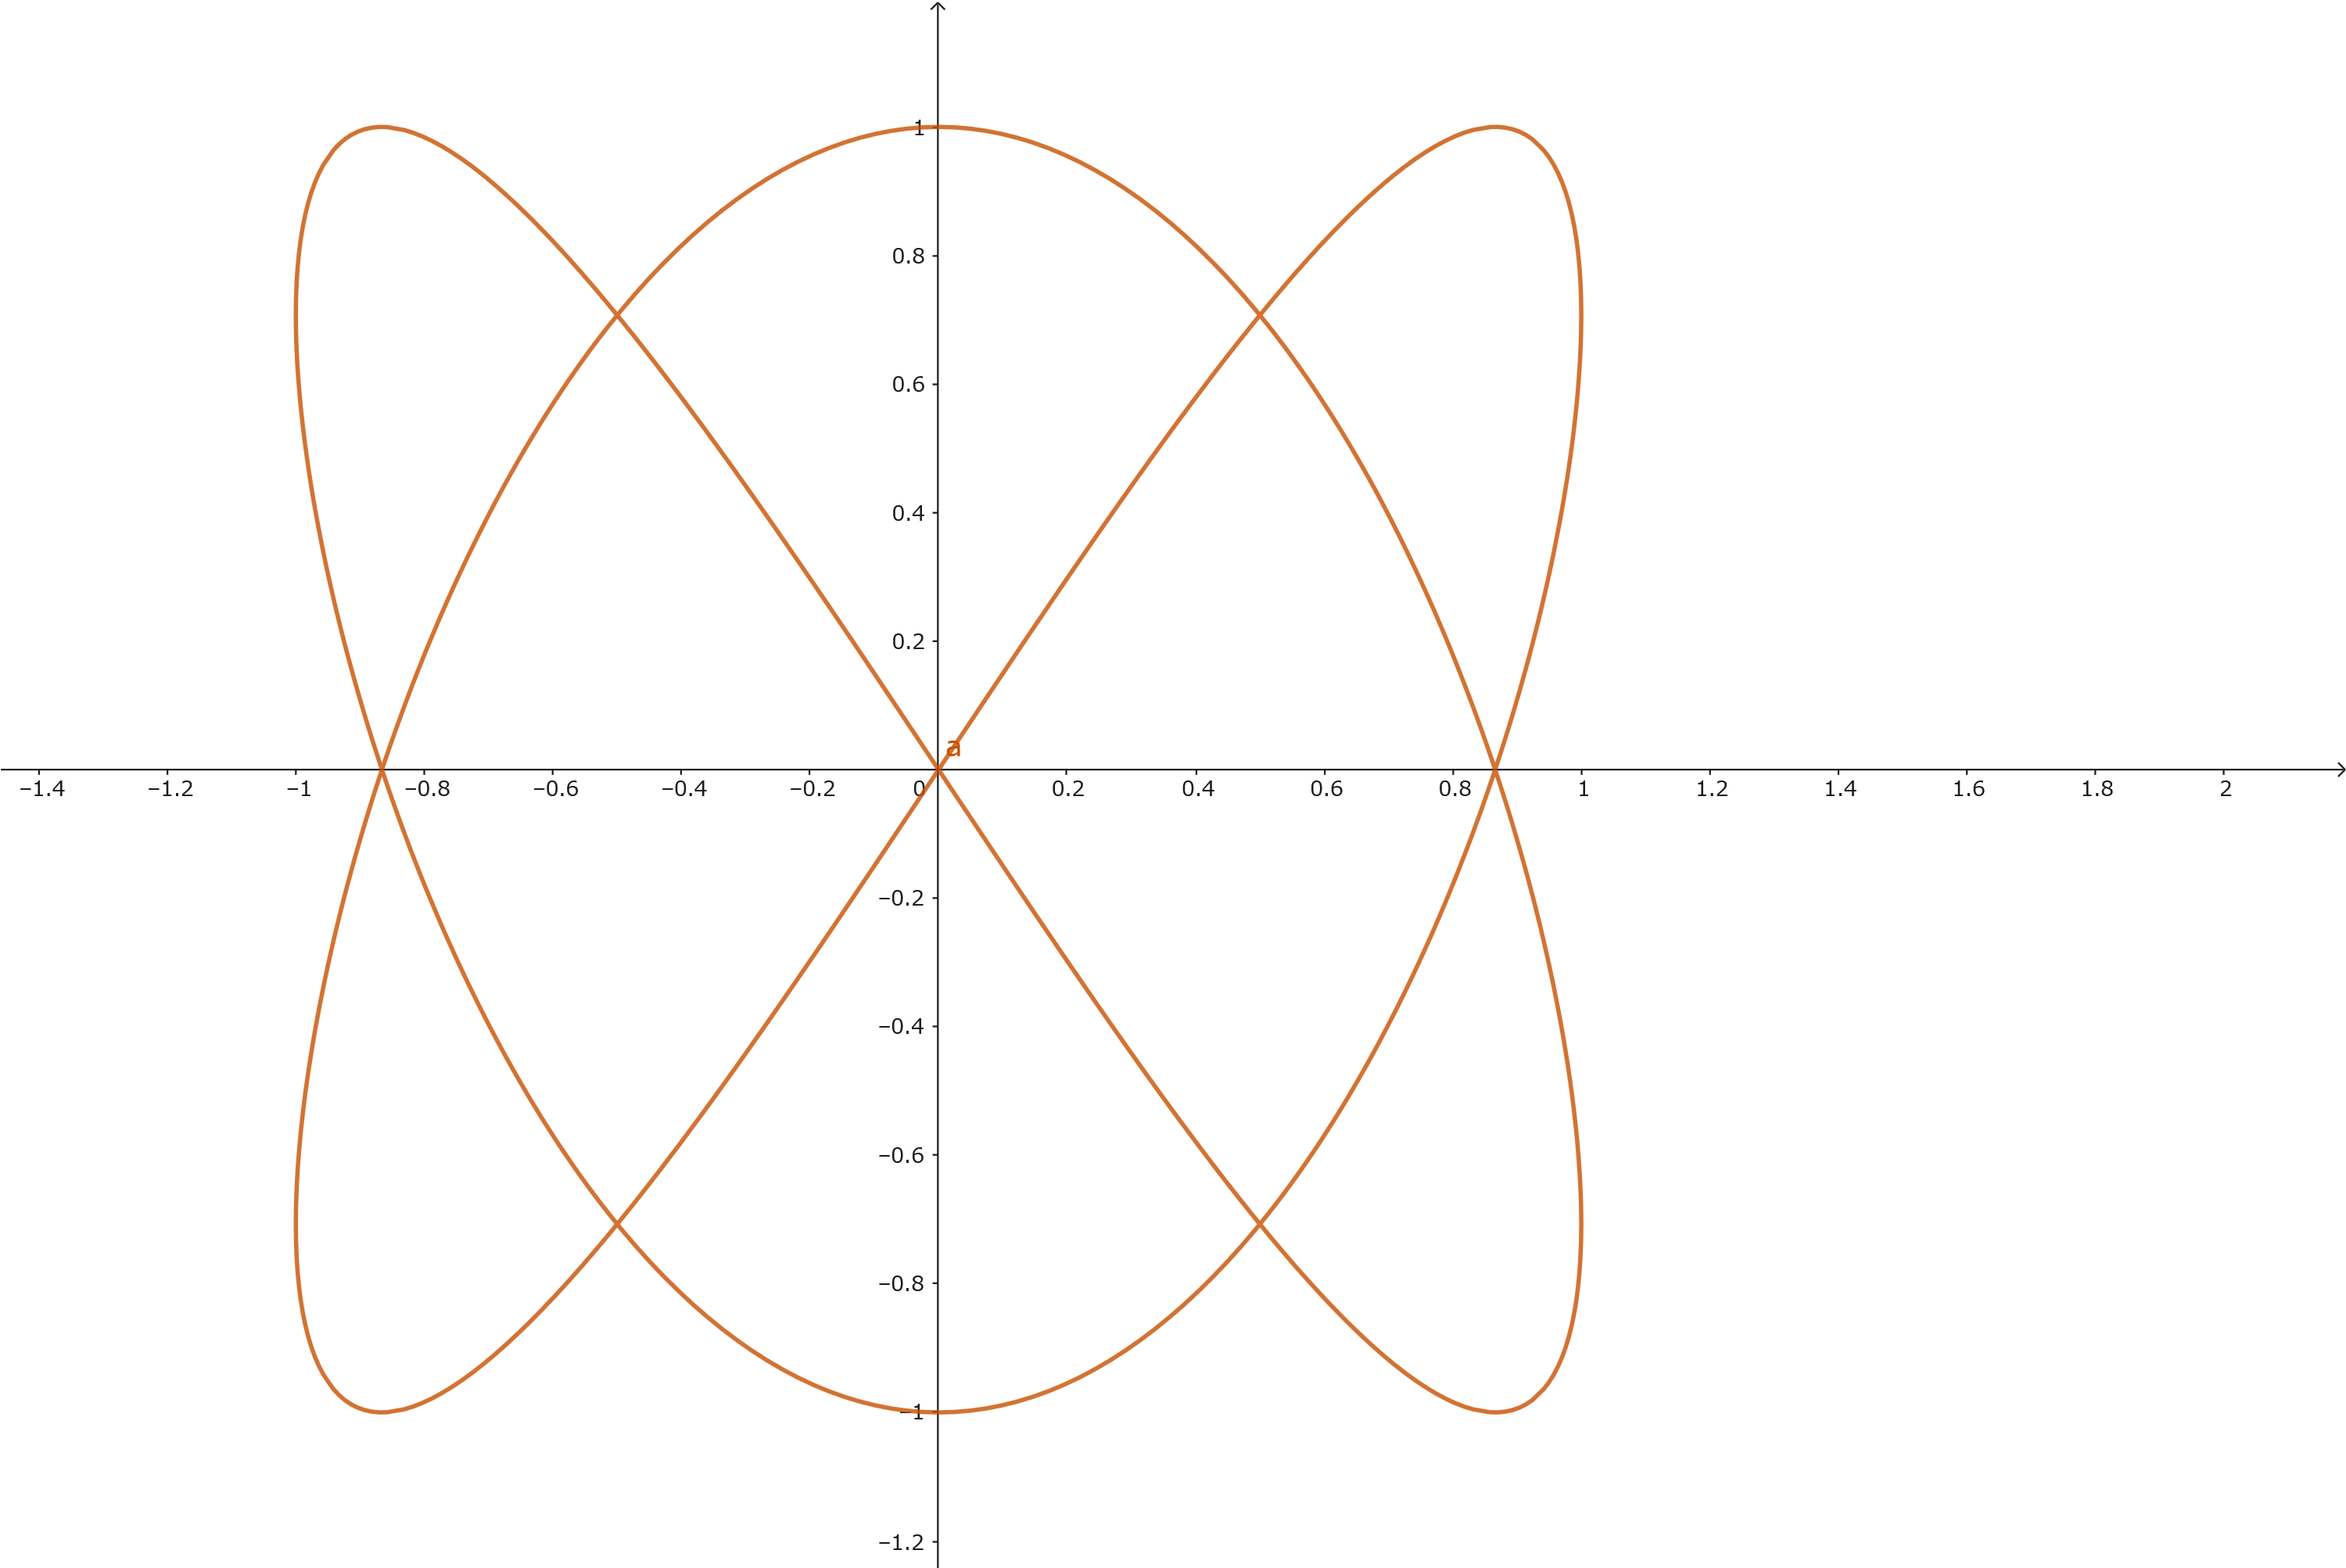
\includegraphics[width=\linewidth]{img/lissajous.png}
  \caption{リサージュ曲線($m=2,n=3$)(generated by GeoGebra)}
\end{figure}
とてもきれいですね。
電通大の校章にも使われているようです\footnote{
  https://www.uec.ac.jp/about/profile/emblem.html
}。
このように閉曲線は、自己交叉することを許可しています。
そうでないような閉曲線は名前がついています。
\begin{definition}
  平面閉曲線$(\gamma,[a,b])$が任意の$a\leq t_1<t_2\leq b$に対して$\gamma(t_1)\neq\gamma(t_2)$を満たす時、\textbf{単純閉曲線}と呼ぶ。
\end{definition}



\section{閉曲線の回転数}

リサージュ曲線のように、ぐるぐると回りまわる閉曲線には、その「\textbf{回転した回数}」が気になるところです。
絵に描いて目に見える曲線なら、それを指でなぞって数えることができますが、そうではない閉曲線にも一般に定義したいところです。

一つの考えとしては、単位接ベクトル$e_1(s)$が定義域を動くとき、これが何周したかを数えることです。
$e_1(s)$の挙動に注目すると、まず$|e_1(s)|=1$なので、$e_1$はよく考えたら円周$S^1$への写像になっています。
\begin{definition}[接線写像]
  $(\gamma,I)$を弧長パラメータ付け可能な平面曲線とし、$s=s(t)$をその弧長パラメータとする。
  このとき、写像
  \[
    e_1:s(I)\to S^1;s\mapsto e_1(s):=\frac{d\gamma(t(s))}{ds}
  \]
  を\textbf{接線写像}という。
\end{definition}

接線写像が$S^1$への写像なので、閉曲線の単位接ベクトルが$S^1$を何周したかは頑張れば定義できそうです。
それは間違いなく、僕たちが知りたい回転数になるはずです。
発想は単純ですが、これを一般論に昇華するためには、基本群で学んだ被覆空間の理論を思い出してほしいです。

\subsection{被覆空間の理論概要}
\begin{definition}[被覆空間]
  $X,\overline{X}$を位相空間とする。
  連続写像$p:\overline{X}\to X$が\textbf{被覆写像}であるとは、任意の$x\in X$に対して、$X$の開集合$U$が存在して、以下を満たす。
  \begin{itemize}
    \item $x\in U$
    \item 開集合$p^{-1}(U)$は、$p$によって$U$と同相な開集合の非交和である。
  \end{itemize}
  $p:\overline{X}\to X$が被覆写像であるとき、$\overline{X}$は$X$の\textbf{被覆空間}であるという。
\end{definition}
\begin{example}
  \[
    p:\mathbb{R}\to S^1;x\mapsto(\cos(x),\sin(x))
  \]
  は被覆写像である。
\end{example}

\begin{definition}
  $X,\overline{X},Y$を位相空間、$p:\overline{X}\to X$を被覆写像、$f:Y\to X$を連続写像とする。
  このとき、連続写像$\overline{f}:Y\to\overline{X}$であって、$p\circ\overline{f}=f$を満たすものを、連続写像$f$の$\overline{X}$への\textbf{持ち上げ}と呼ぶ。
\end{definition}
\begin{theorem}[道の持ち上げ定理]
  $X,\overline{X}$を位相空間、$p:\overline{X}\to X$を被覆写像、$I\subset\mathbb{R}$を閉区間、$f:I\to X$を連続写像とする。
  このとき、$f$の$\overline{X}$への持ち上げ$\overline{f}:I\to\overline{X}$が存在する。
\end{theorem}
\begin{example}
  $(\gamma,I)$を弧長パラメータ付け可能な平面曲線とし、$s=s(t)$をその弧長パラメータとする。
  このとき、接線写像
  \[
    e_1:s(I)\to S^1;s\mapsto e_1(s)=\frac{d\gamma(t(s))}{ds}
  \]
  は連続写像である。
  従って、接線写像の$\mathbb{R}$への持ち上げ
  \[
    \overline{e_1}:s(I)\to\mathbb{R}
  \]
  が存在する。
\end{example}

\begin{definition}[被覆変換群]
  $X,\overline{X}$を位相空間、$p:\overline{X}\to X$を被覆写像とする。
  このとき、同相写像$f:\overline{X}\to\overline{X}$であって、$p\circ f=p$を満たすものを\textbf{被覆変換}と呼ぶ。
\end{definition}
\begin{theorem}
  $X,\overline{X}$を位相空間、$p:\overline{X}\to X$を被覆写像とする。
  このとき、被覆変換全体の集合
  \[
    \operatorname{Aut}_X(\overline{X}):=\{f:\overline{X}\overset{\cong}{\longrightarrow}\overline{X}\mid p\circ f=p\}
  \]
  は、写像の合成によって群となる。
\end{theorem}
\begin{example}
  \[
    \operatorname{Aut}_{S^1}(\mathbb{R})\cong\mathbb{Z};f\mapsto \frac{f(0)}{2\pi}
  \]
  となる。実際、被覆変換は$p\circ f=f$を満たすために$f(x)=x+2\pi n$という形しか取れない。
\end{example}

\subsection{回転数}

被覆写像$p:\mathbb{R}\to S^1$に対する被覆変換群は、イメージとしては常螺旋を一段ずつ上にあげたり下げたりする操作を表わします。
一方で$\operatorname{Aut}_{S^1}(\mathbb{R})\cong\mathbb{Z}$は被覆空間に関するガロア対応によって、$S^1$の\textbf{基本群}$\pi_1(S^1)$と同型でした。
$\pi_1(S^1)\cong\mathbb{Z}$の元は、ざっくり言って「$n$回$S^1$を回る道の代表元」なのでした。
これを結びつけて行けば、被覆変換の「何段変わったか？」のイメージを閉曲線の回転数に採用できそうです。
\begin{definition}
  $(\gamma,I)$を弧長パラメータ付け可能な閉曲線とし、$s=s(t)$をその弧長パラメータとする。
  $e_1(s)$を$\gamma$の単位接ベクトルとし、これを接線写像$e_1:s(I)\to S^1$とみたときの$\mathbb{R}$への持ち上げを$\overline{e_1}:s(I)\to\mathbb{R}$とおく。
  また、$s(I)=[0,L]$であるとする(すなわち$\gamma$の長さを$L$とする)。
  \[
    w_\gamma:=\frac{\overline{e_1}(L)-\overline{e_1}(0)}{2\pi}
  \]
  を$(\gamma,I)$の\textbf{回転数}と呼ぶ。
\end{definition}
この定義でもたらされた回転数が整数であることは、被覆変換群の理論からしっかり保証されています！
\begin{figure}[htbp]
  \centering
  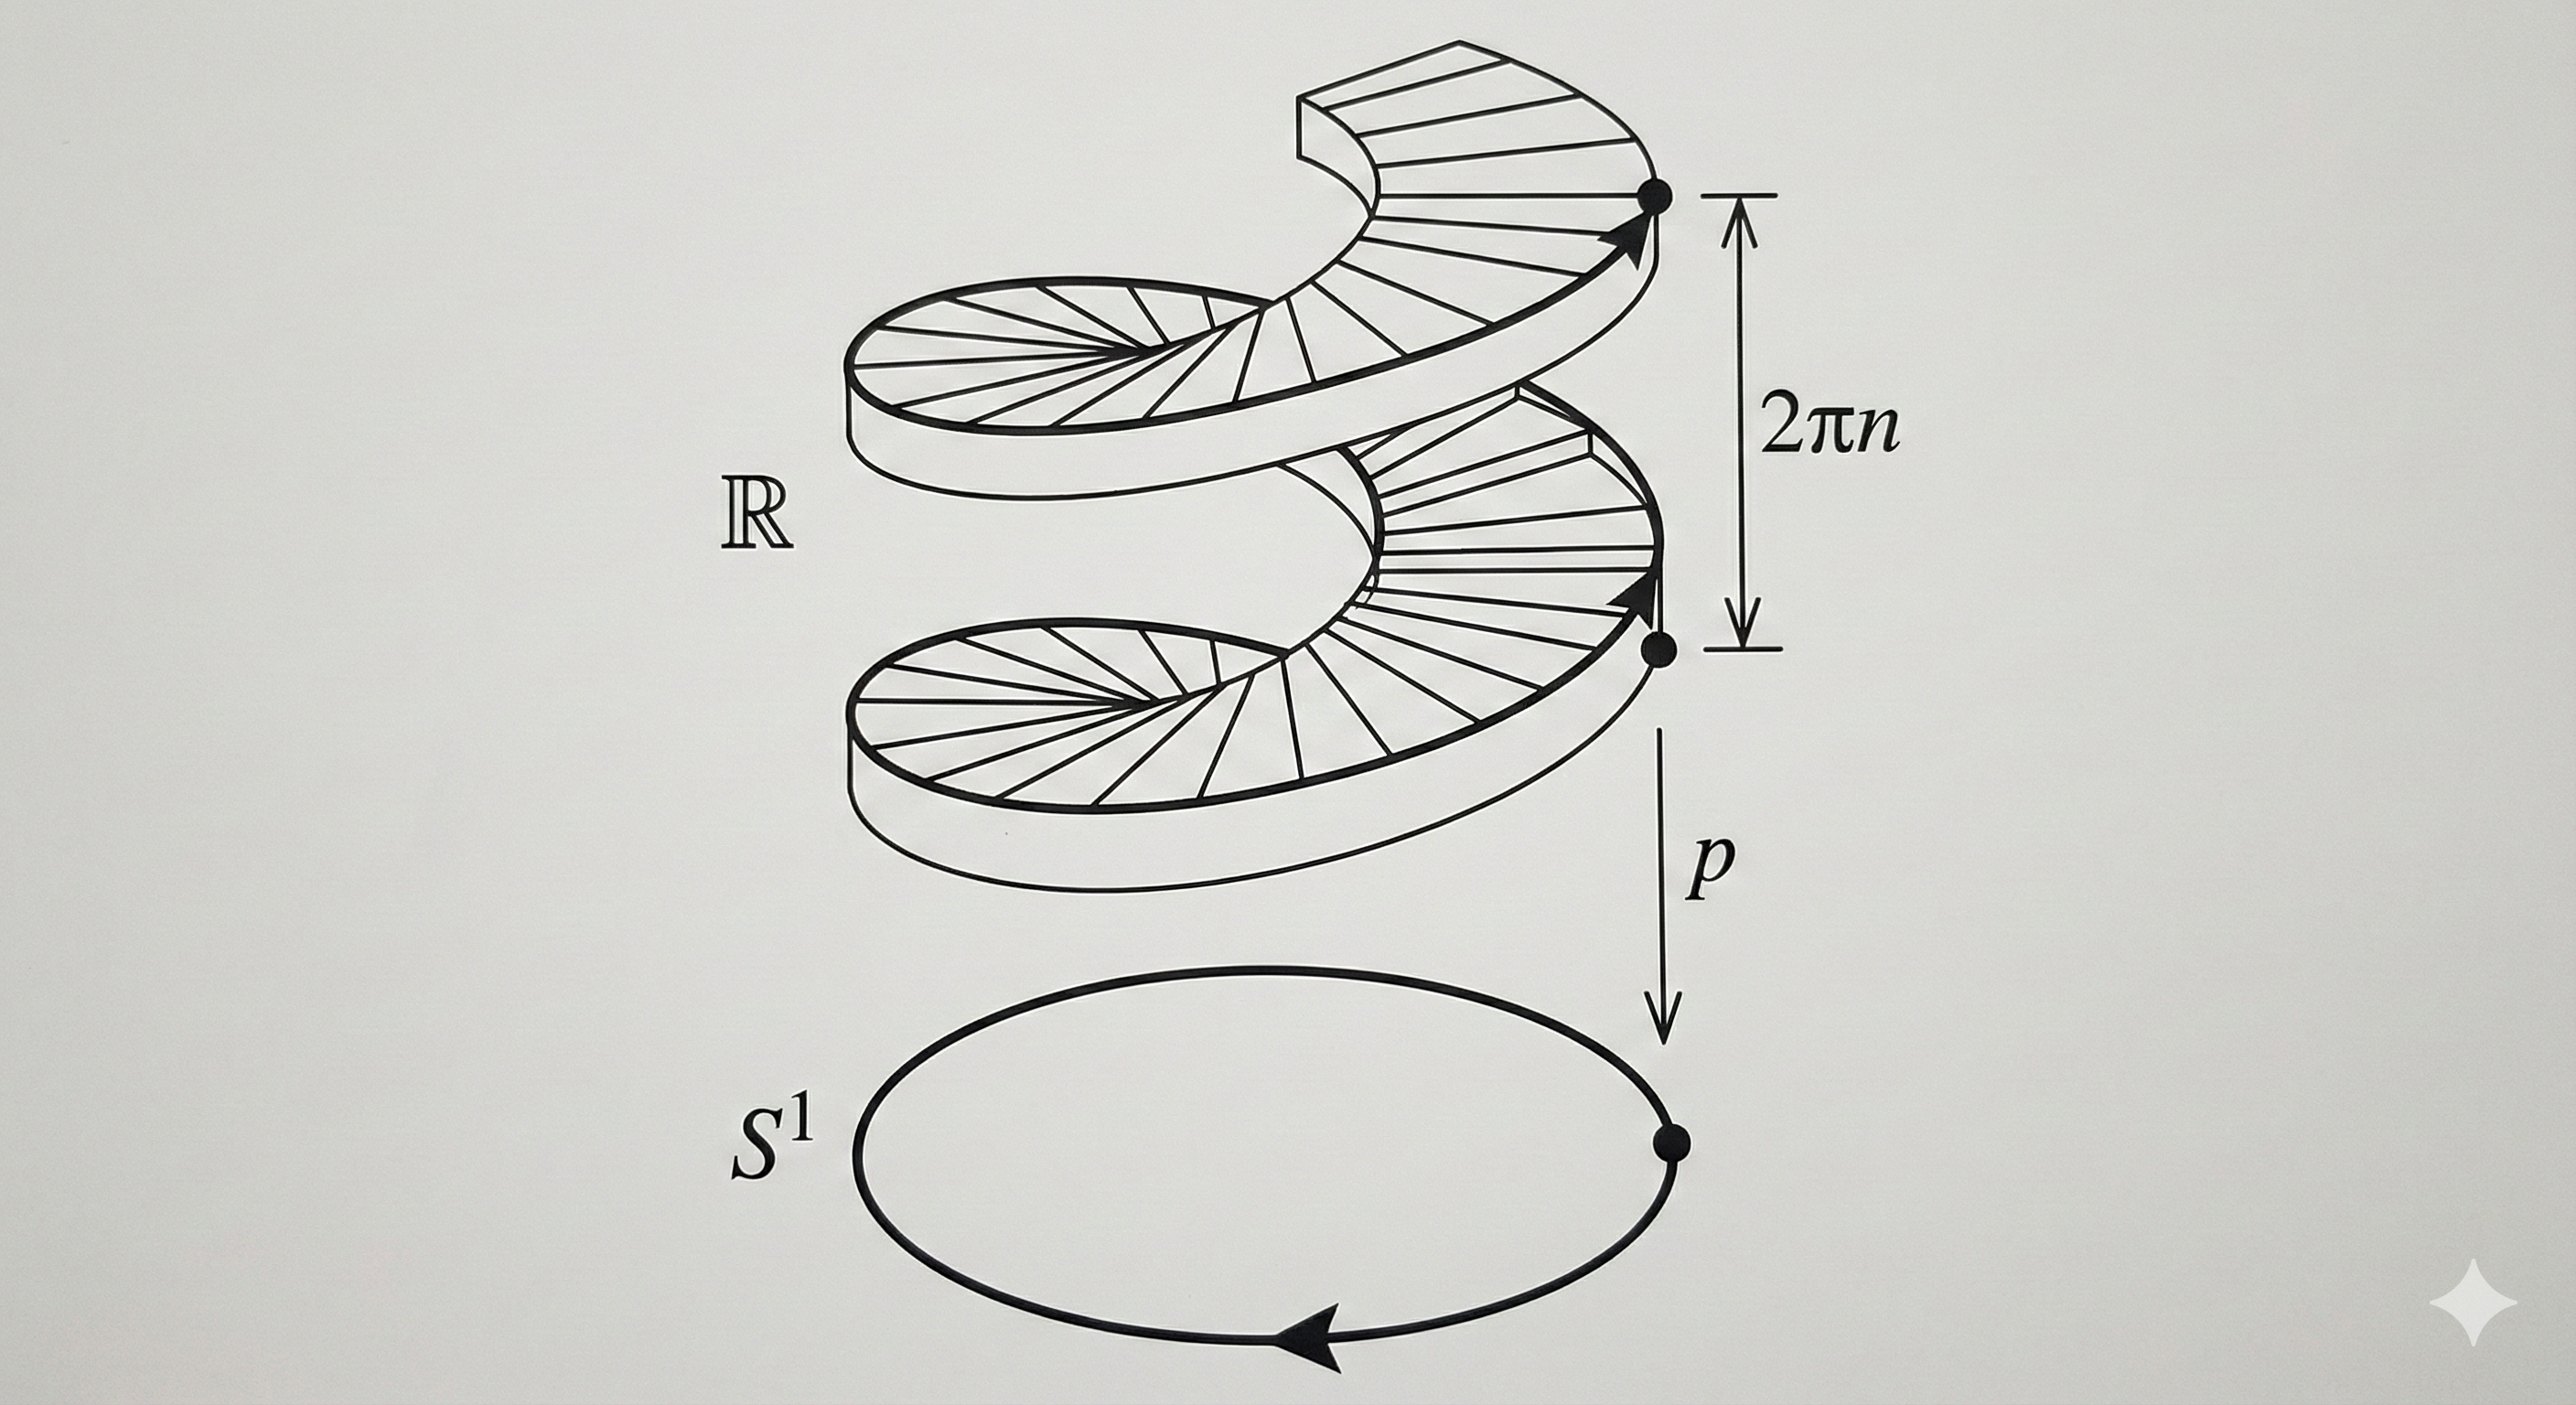
\includegraphics[width=\linewidth]{img/Gemini_Generated_Image_2isokk2isokk2iso.png}
  \caption{回転数のイメージ(generated by Gemini)}
\end{figure}

\subsection{回転数の計算例}

分かり切った計算ですが、円の回転数を求めてみましょう。
\begin{example}
  弧長パラメータ付けた円$\gamma(t(s))=(\cos(s),\sin(s))$に対して、$e_1(s)=(-\sin(s),\cos(s))$。
  接線写像とみた$e_1:[0,2\pi]\to S^1$の被覆写像$p:\mathbb{R}\to S^1;x\mapsto(\cos(x),\sin(x))$への持ち上げは、例えば
  \[
    \overline{e_1}(s)=s+\frac{\pi}{2}
  \]
  となる。
  ゆえに
  \[
    w_\gamma=\frac{\overline{e_1}(2\pi)-\overline{e_1}(0)}{2\pi}=\frac{(2\pi+\pi/2)-\pi/2}{2\pi}=1
  \]
  となる。
\end{example}
思った通りですね。

ここで残念なお知らせです。
ろくに定義から計算できる閉曲線はこれぐらいです。
なぜなら、単位接ベクトル$e_1(s)$を求めるということは、ほとんどの曲線では重労働だからです。
これは弧長パラメータの求めにくさから来ています。
例えば楕円$\gamma(t)=(a\cos(t),b\sin(t))$でさえ、その弧長は楕円積分という積分の実行が不可能な形になるのでした。
なので、もう少し議論を進めていく必要がありそうです。

\subsection{回転数と曲率の積分との関係}

まず
\[
  \overline{e_1}(L)-\overline{e_1}(0)
\]
がどんな形で表わせそうに見えますか？
例えば
\[
  \overline{e_1}(s)=\int_0^s f(\xi)d\xi
\]
という関数$f(x)$、つまり$\overline{e_1}:[0,L]\to\mathbb{R}$の原始関数があれば
\[
  \overline{e_1}(L)-\overline{e_1}(0)=\int_0^Lf(\xi)d\xi
\]
と表わせるはずです。
$f(x)$を求めるためには、$\overline{e_1}(s)=\int_0^s f(\xi)d\xi$の両辺を微分するしかないですね。
微分可能かどうかは一旦おいておいて、まずやってみましょう。
\[
  f(s)=\frac{d\overline{e_1}(s)}{ds}
\]

まだよくわからないということで、被覆写像$p:\mathbb{R}\to S^1;t\to(\cos(t),\sin(t))$を合成してみましょう。
\[
  p(f(s))=p\left(\frac{d\overline{e_1}(s)}{ds}\right)
\]
これも手が止まってしまいそうです。

もっと手前に戻りましょう。
$\overline{e_1}(s)$は$e_1(s)=p(\overline{e_1}(s))$を満たすような持ち上げでした。
この両辺を微分すれば、合成関数の微分法則から$d\overline{e_1}(s)/ds$が出てくるはずです！
\[
  \frac{de_1(s)}{ds}=\frac{dp(\overline{e_1}(s))}{ds}=\frac{d(\cos(\overline{e_1}(s)),\sin(\overline{e_1}(s)))}{ds}=\frac{d\overline{e_1}(s)}{ds}(-\sin(\overline{e_1}(s)),\cos(\overline{e_1}(s)))
\]
左辺の絶対値は空間曲線で定義した曲率$\kappa(s)$にほかなりません！
また右辺の因子のうち、
\[
  e_2(s):=(-\sin(\overline{e_1}(s)),\cos(\overline{e_1}(s)))
\]
は$e_1(s)$と直交する単位法線ベクトルになっています。
実際、長さが1になることは自明です。
また、$e_1=p\circ\overline{e_1}$であったから、実は
\[
  e_1(s)=p(\overline{e_1})=(\cos(\overline{e_1}),\sin(\overline{e_1}))
\]
と書き表せるからです。

さて、ここで一つの問題が発生します。
空間曲線の曲率は$\kappa(s)=|d^2\gamma(t(s))/ds^2|$でしたので、得られた等式
\[
  \frac{de_1(s)}{ds}=\frac{d\overline{e_1}(s)}{ds}e_2(s)
\]
から、
\[
  \kappa(s)=\left|\frac{d\overline{e_1}(s)}{ds}\right|
\]
というどこか惜しい式が出てきました。
符号が正で取れればうれしいのに…。

そこで空間曲線では、そもそもなぜ$\kappa(s)>0$となっていたことを思い出しましょう。
これは定義としては
\[
  \kappa(s):=\left|\frac{de_1(s)}{ds}\right|
\]
で平面曲線と同様なのですが、最大の目的は主法線ベクトル$e_2(s)$を定義
\[
  e_2(s):=\frac{de_1(s)/ds}{|de_1(s)/ds|}
\]
において、0除算を避けるためでした。

ところが平面曲線の場合、このような0除算を避けて法線ベクトル$e_2(s)$が先ほどの通り
\[
  e_2(s):=(-\sin(\overline{e_1}(s)),\cos(\overline{e_1}(s)))
\]
と定義されました。
であれば、そもそも曲率と呼ぶべき
\[
  \kappa(s)=\left|\frac{de_1(s)}{ds}\right|
\]
が絶対に正でなければいけないという理由もないです。
逆に自然に
\[
  \kappa_p(s)=\frac{d\overline{e_1}(s)}{ds}
\]
こそが曲率であると考えてよかろうなのです(平面(plane)の$p$を添え字につけておきました)。
であれば、次がなりたつということです！
\begin{theorem}
  $(\gamma,I)$を弧長パラメータ付け可能な閉曲線とし、$s=s(t)$をその弧長パラメータとする。
  $e_1(s)$を$\gamma$の単位接ベクトルとし、これを接線写像$e_1:s(I)\to S^1$とみたときの$\mathbb{R}$への持ち上げを$\overline{e_1}:s(I)\to\mathbb{R}$とおく。
  また、$s(I)=[0,L]$であるとする。
  このとき、次が成り立つ。
  \[
    w_\gamma=\frac1{2\pi}\int_0^L\kappa_p(s)ds
  \]
\end{theorem}
こうなるとこの関数が、以前にやった「接円の半径の逆数」としての意味をどのように持っているかが気になってくるところです。
簡単な例でいくつか確認しましょう。

\begin{example}
  半径$r>0$の円
  \[
    \gamma:[0,2\pi]\to\mathbb{R}^2;t\mapsto r(\cos(t),\sin(t))
  \]
  について考える。このとき弧長パラメータは$s(t)=rt\Leftrightarrow t(s)=s/r$である。
  ゆえに$\gamma(t(s))=r(\cos(s/r),\sin(s/r))$であり、$e_1(s)=(-\sin(s/r),\cos(s/r))$となる。
  これを$\gamma$の接線写像$e_1:[0,2\pi r]\to S^1$とみたとき、被覆空間$\mathbb{R}\to S^1;x\mapsto(\cos(x),\sin(x))$への持ち上げは、
  \[
    \overline{e_1}(s)=\frac{s}{r}+\frac{\pi}{2}
  \]
  となる。
  ゆえに平面曲線の曲率は
  \[
    \kappa_p(s)=\frac{d\overline{e_1}(s)}{ds}=\frac{1}{r}
  \]
  となり、空間曲線の曲率と一致する。

  一方で、逆回りの円
  \[
    \gamma:[0,2\pi]\to\mathbb{R}^2;t\mapsto r(\cos(-t),\sin(-t))
  \]
  について考える。このとき弧長パラメータは変わらず、$s(t)=rt\Leftrightarrow t(s)=s/r$である。
  ゆえに$\gamma(t(s))=r(\cos(-s/r),\sin(-s/r))$であり、$e_1(s)=(\sin(-s/r),-\cos(-s/r))$となる。
  これを$\gamma$の接線写像$e_1:[0,2\pi r]\to S^1$とみたとき、被覆空間$\mathbb{R}\to S^1;x\mapsto(\cos(x),\sin(x))$への持ち上げは、
  \[
    \overline{e_1}(s)=-\frac{s}{r}-\frac{\pi}{2}
  \]
  となる。
  ゆえに平面曲線の曲率は
  \[
    \kappa_p(s)=\frac{d\overline{e_1}(s)}{ds}=-\frac{1}{r}
  \]
  となる。
  これは空間曲線の曲率とは符号のみ異なる。
\end{example}
これは平面においては、曲線が時計回りか反時計回りかを、曲率によって区別することができることを意味します。
空間においては、その曲線をどこから見れば時計回りか反時計回りかが、実は区別できないです。
$z$軸の上から見れば時計回りな円でも、$z$軸の下から見れば反時計回りになります。
一方で平面曲線は、\textbf{その二次元の世界に住んでいる人々から見れば}、その曲線が時計回りか反時計回りかは一意に判別できるのです。
このような見え方の違いが、平面曲線と空間曲線で異なるのです。

遅ればせながら、平面曲線の曲率を定義しましょう。
\begin{definition}
  $(\gamma,I)$を平面曲線かつ閉曲線、$s=s(t)$をその弧長パラメータとする。
  $L$を$(\gamma,I)$の弧長とし、$e_1:[0,L]\to S^1;s\mapsto d\gamma(t(s))/ds$を接線写像とする。
  $p:\mathbb{R}\to S^1;x\mapsto(\cos(x),\sin(x))$を$S^1$の被覆写像とする。
  このとき、
  \[
    \kappa_p(s)=\frac{d\overline{e_1}(s)}{ds}
  \]
  を、曲線$(\gamma,I)$の\textbf{平面曲率}と呼ぶ。
\end{definition}

実際のところ、接線写像$e_1$の持ち上げ$\overline{e_1}$が微分可能かどうかはまだ証明していませんでした。
面倒ですが、まあ頑張って証明しましょう。
\begin{theorem}
  $(\gamma,I)$を平面曲線かつ閉曲線、$s=s(t)$をその弧長パラメータとする。
  $L$を$(\gamma,I)$の弧長とし、$e_1:[0,L]\to S^1;s\mapsto d\gamma(t(s))/ds$を接線写像とする。
  $p:\mathbb{R}\to S^1;x\mapsto(\cos(x),\sin(x))$を$S^1$の被覆写像とする。
  このとき、接線写像$e_1$の$\mathbb{R}$への持ち上げ$\overline{e_1}:[0,L]\to\mathbb{R}$は$C^1$級である。
\end{theorem}
\begin{proof}
  まず$s\in(0,L)$に対して、$p:\mathbb{R}\to S^1$は被覆写像であるから、$e_1(s)\in S^1$を含む開集合$U\subset S^1$が存在して、$p^{-1}(U)$は被覆写像$p$によって同相な開集合の非交和である。
  より小さく$U$をとって、十分小さな$\delta>0$に対して、
  \[
    U=\{(\cos(x),\sin(x))\mid |x-\overline{e_1}(s)|<\delta\}
  \]
  であるとしてよい。
  このとき$p^{-1}(U)$は、$n\in\mathbb{Z}$に対して$V_n:=\{x+2\pi n\mid |x-\overline{e_1}(s)|<\delta\}$とおけば
  \[
    p^{-1}(U)=\bigsqcup_{n\in\mathbb{Z}}V_n
  \]
  である。

  $\overline{e_1}(s)\in V_0$であるから、$V_0$に注目すると、$u\in V_0$に対して
  \[
    p|_{V_0}(u)=(\cos(u),\sin(u))
  \]
  である。
  ここで、$\gamma(t(u))=(f(u),g(u))$とおくと、$e_1(u)=d\gamma(t(u))/du$。
  また$p\circ\overline{e_1}(u)=e_1(u)$より、
  \[
    p(\overline{e_1}(u))=e_1(u)=\left(\frac{df(u)}{du},\frac{dg(u)}{du}\right)
  \]
  左辺は$(\cos(\overline{e_1}(u)),\sin(\overline{e_1}(u)))$に他ならないから、
  \[
    \begin{cases}
      \cos(\overline{e_1}(u))=\frac{df(u)}{du}\\
      \sin(\overline{e_1}(u))=\frac{dg(u)}{du}
    \end{cases}
  \]
  以下、$e_1(s)$の位置によって場合分けを行う。

  \textbf{$\cos(\overline{e_1}(s))\neq0$の場合。}
  このとき$\sin(\overline{e_1}(s))\neq\pm1$である。
  従って、必要ならばさらに$\delta>0$を小さく取り、任意の$u\in V_0$に対して
  \[
    \sin(\overline{e_1}(u))\in(0,1)
  \]
  は単調増加、あるいは単調減少であるとしてよい($\sin$のグラフを思い浮かべよ)。
  この範囲で、$\arcsin$は$C^\infty$級関数であり、
  \[
    \overline{e_1}(u)=\arcsin\left(\frac{dg(u)}{du}\right)+2k\pi
  \]
  が得られる。
  $\gamma$は$C^2$級だったから、$dg(u)/du$は$C^1$級である。
  ゆえに$\overline{e_1}(u)=\arcsin\left(\frac{dg(u)}{du}\right)+2k\pi$は$C^1$級であって、これが求めたいことであった。

  \textbf{$\cos(\overline{e_1})(s)=0$の場合。}
  このとき、必要ならばさらに$\delta>0$を小さく取り、任意の$u\in V_0$に対して
  \[
    \cos(\overline{e_1}(u))\in(0,1)
  \]
  は単調増加、あるいは単調減少であるとしてよい($\cos$のグラフを思い浮かべよ)。
  この範囲で、$\arccos$は$C^\infty$級関数であり、
  \[
    \overline{e_1}(u)=\arccos\left(\frac{df(u)}{du}\right)+2k\pi
  \]
  $\gamma$は$C^2$級だったから、$df(u)/du$は$C^1$級である。
  ゆえに$\overline{e_1}(u)=\arccos\left(\frac{df(u)}{du}\right)+2k\pi$は$C^1$級であって、これが求めたいことであった。
\end{proof}



\section{回転数と平面曲率の関係式の使用例}

平面曲線$(\gamma,I)$の平面曲率$\kappa_p:s(I)\to\mathbb{R}$の定義はとても複雑でした。
あらためて手順を説明すると、
\begin{enumerate}
  \item 弧長パラメータ$s=s(t)$を用意する
  \item 全弧長$L$を求める
  \item 単位接ベクトル$e_1$を接線写像$e_1:[0,L]\to S^1$とみる
  \item $S^1$には被覆空間$p:\mathbb{R}\to S^1;t\mapsto(\cos(t),\sin(t))$があった
  \item 接線写像$e_1$の$\mathbb{R}$への持ち上げ$\overline{e_1}:[0,L]\to\mathbb{R}$は$C^1$級
  \item このとき、平面曲率は
  \[
    \kappa_p:[0,L]\to\mathbb{R};s\mapsto\frac{d\overline{e_1}(s)}{ds}
  \]
  で定義される。
\end{enumerate}
このとき、$\gamma$の回転数$w_\gamma$は
\[
  w_\gamma=\frac1{2\pi}\int_0^L\kappa_p(s)ds
\]
で求められるのでした。
$\kappa_p(s)$という局所的に定義したものを積分が$2\pi$の整数倍になるのが驚きですね。
しかもその整数というのが、位相的には見た目で計算できる回転数になるのは凄いと思います。
例えば楕円
\[
  \gamma(t)=(a\cos(t),b\sin(t))
\]
で上の手順で$\int\kappa_p(s)ds$を求めようとするとめちゃくちゃ大変ですが、もう$S^1$と同相なので
\[
  \int_0^L\kappa_p(s)ds=2\pi w_{\text{楕円}}=2\pi
\]
と求まります。

リサージュ曲線の曲率の場合、逆に目で追うのが大変ですが、$\kappa_p$を積分することで0になることがわかります。
実は(例\ref{example:Lissajous_curve}の)リサージュ曲線の回転数はすべて0です。
例えば$(m,n)=(1,2)$のリサージュ曲線はこんな形になります。
\begin{figure}[htbp]
  \centering
  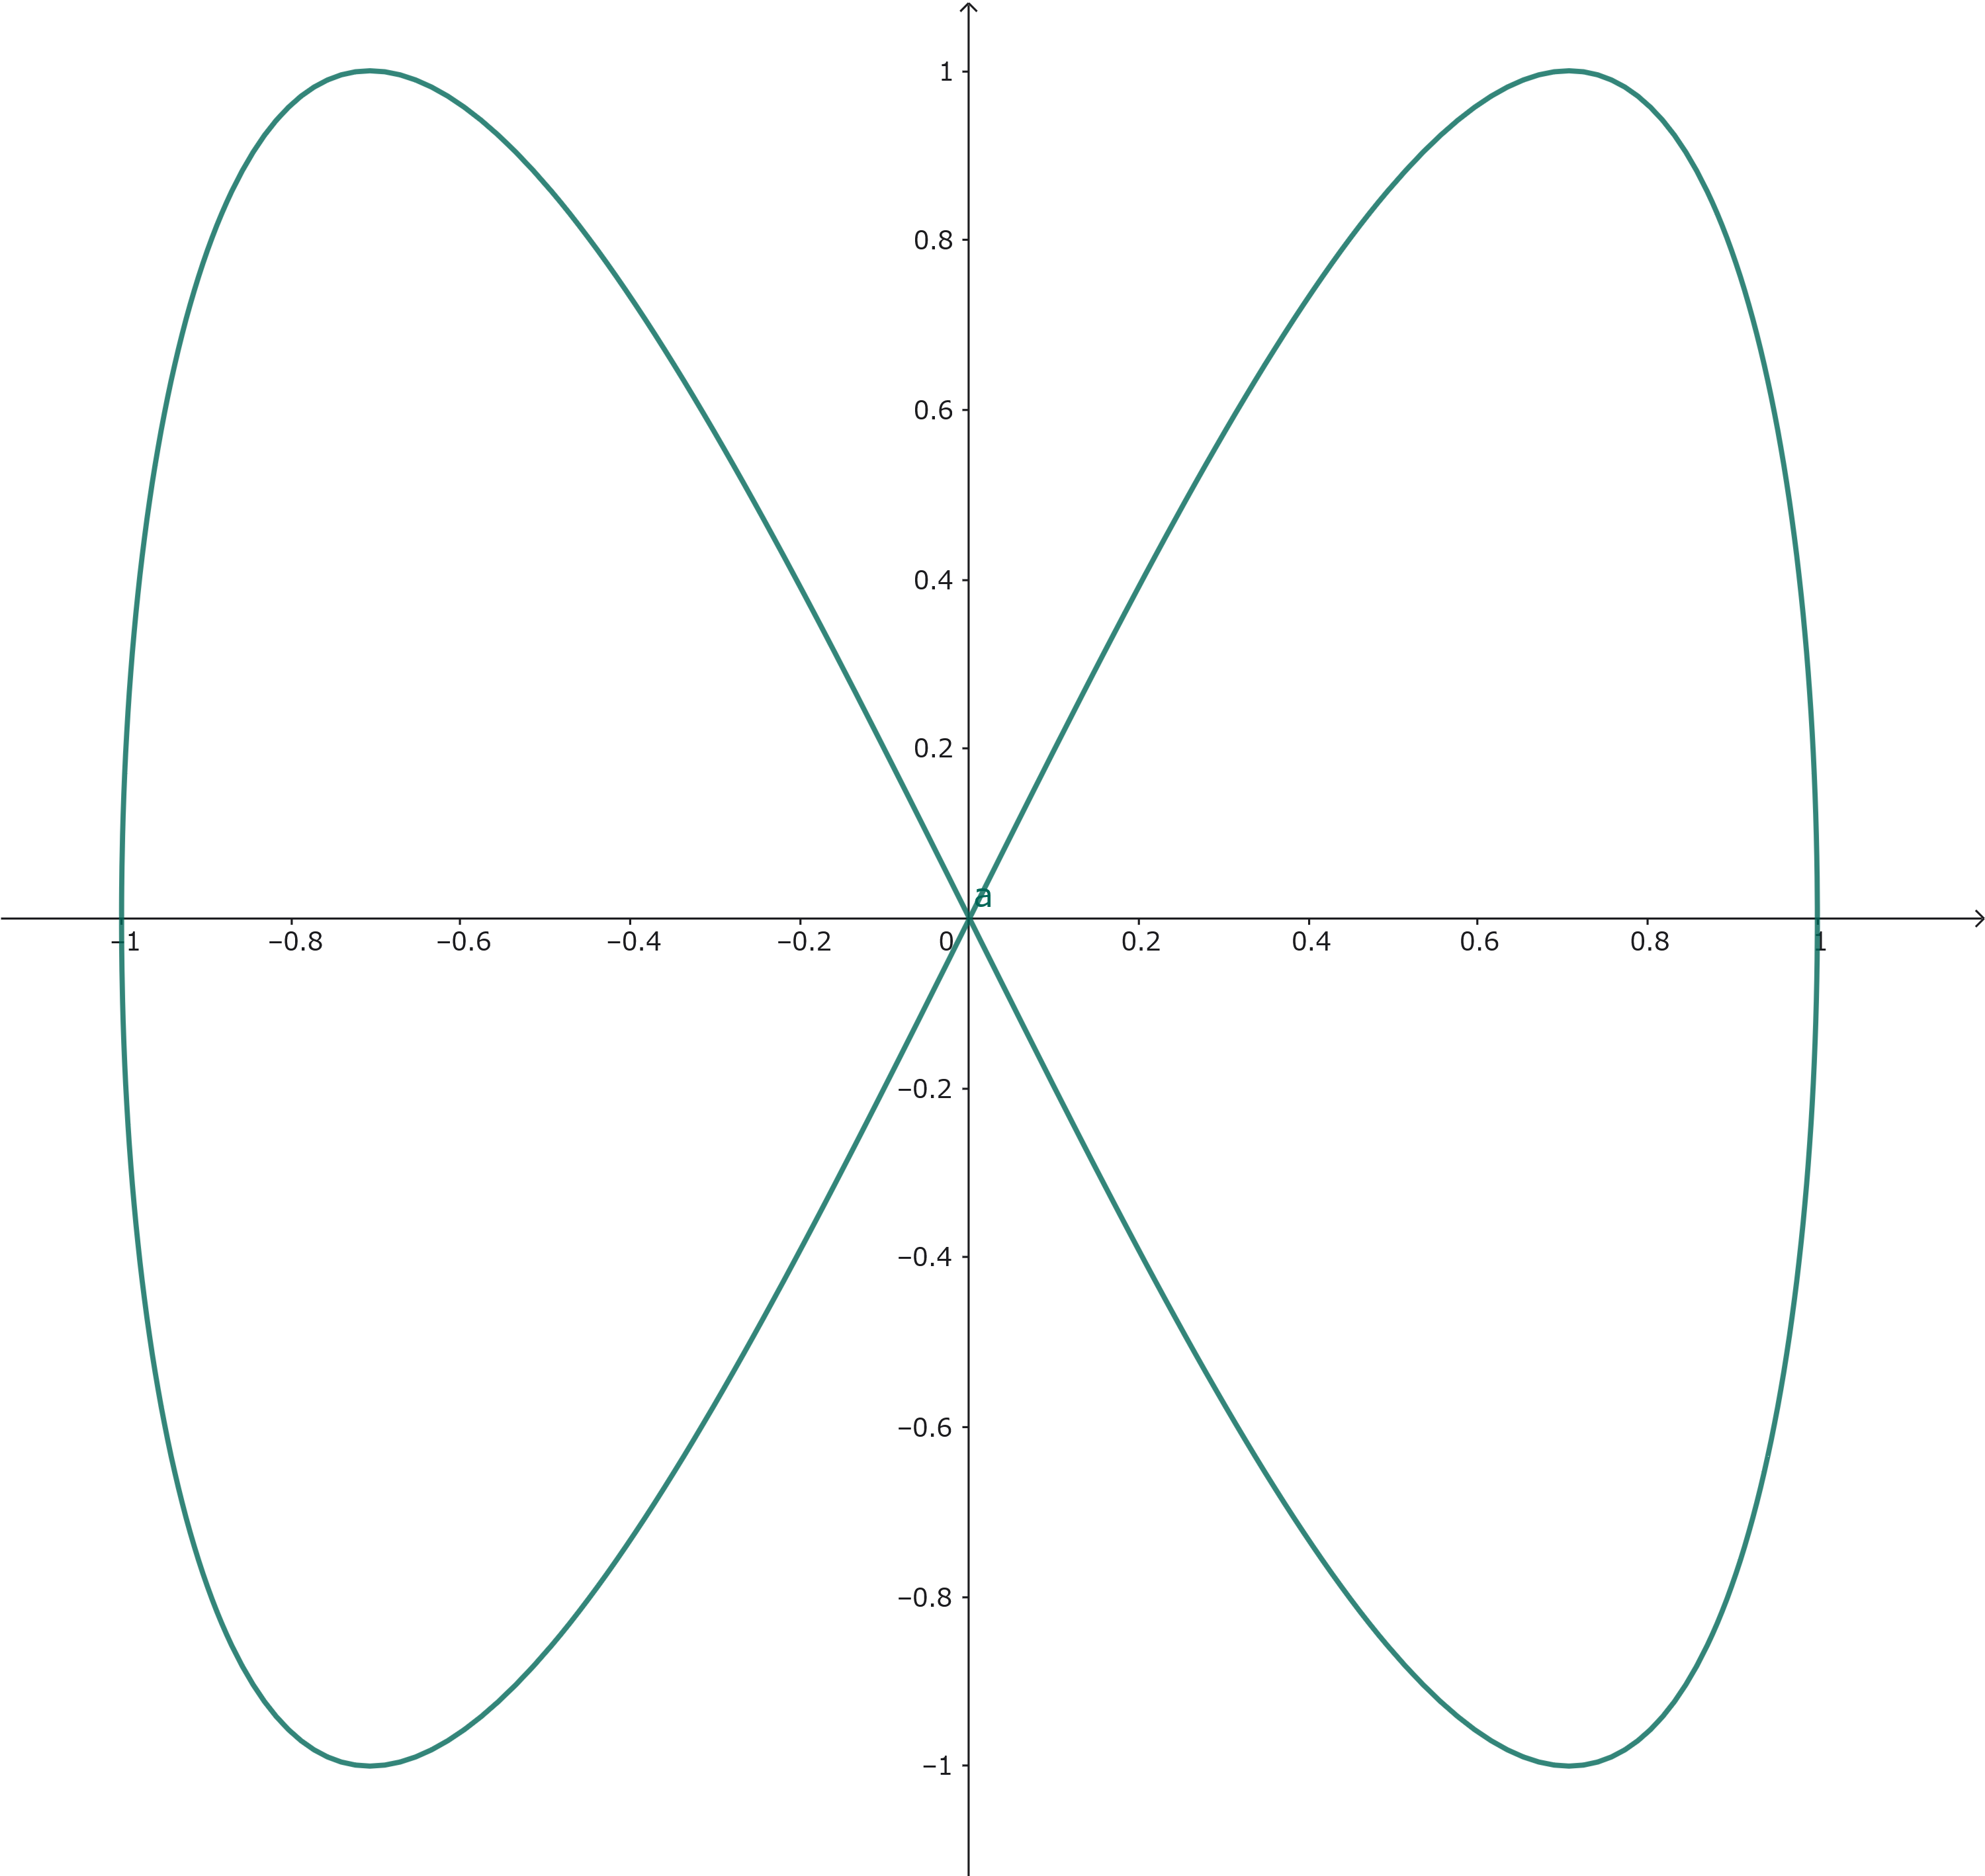
\includegraphics[scale=2.0]{img/Lissajous_curve_1_2.png}
  \caption{($m=1,n=2$)(generated by GeoGebra)}
\end{figure}
マリオカートか何かで、このような形のサーキットがあったと思います。
ともかくこのサーキットで原点から車を走らせると、まず第一象限から第四象限にいる間は、右方向にハンドルを曲げなければいけません。
第四象限を抜けて、第二象限に突入すると、ハンドルを左方向に曲げ無ければいけません。
そして一周して戻ってくる。
合計の回転数は左右が打ち消しあって0というわけです。

一般の場合に示してみましょう。
\begin{theorem}
  $m, n \in \mathbb{Z} \setminus \{0\}$ を互いに素な整数とし、その和 $m+n$ は奇数であるとする（すなわち偶奇が異なる）。
  このとき、閉曲線
  \[
    \gamma: [0, 2\pi] \to \mathbb{R}^2, \quad \gamma(t) = (\sin(mt), \sin(nt))
  \]
  の回転数は $0$ である。
\end{theorem}
\begin{proof}
  まずは平面曲率を求めるために、弧長パラメータを定義しておくと、
  \[
    s(t)=\int_0^t \sqrt{m^2\cos^2(mt)+n^2\cos^2(nt)} \, dt
  \]
  となる。
  すると
  \[
    e_1(s):=\frac{d\gamma(t(s))}{ds}=\frac{dt}{ds}\frac{d\gamma(t)}{dt}=\frac{(m\cos(mt),n\cos(nt))}{\sqrt{m^2\cos^2(mt)+n^2\cos^2(nt)}}
  \]
  となる。
  一旦、このまま$\mathbb{R}$に持ち上げて
  \[
    \overline{e_1}:[0,L]\to\mathbb{R}
  \]
  を作ります。
  このとき、単位接ベクトルと単位法ベクトルは
  \begin{align*}
    e_1(s)&=(\cos(\overline{e_1}(s)),\sin(\overline{e_1}(s)))\\
    e_2(s)&=(-\sin(\overline{e_1}(s)),\cos(\overline{e_1}(s)))
  \end{align*}
  であるから、$de_1(s)/ds$から$d\overline{e_1}(s)/ds=:\kappa_p(s)$が出てくる。
  \[
    \kappa_p(s)=\frac{de_1(s)}{ds}\cdot e_2(s)
  \]
  さらに計算を進めると、$e_1(s)$から結果的に$e_2(s)$の各成分を知ることができる。
  \begin{align*}
    e_1(s)&=(\cos(\overline{e_1}(s)),\sin(\overline{e_1}(s)))=p(\overline{e_1}(s))=\frac{(m\cos(mt),n\cos(nt))}{\sqrt{m^2\cos^2(mt)+n^2\cos^2(nt)}}\\
    e_2(s)&=(-\sin(\overline{e_1}(s)),\cos(\overline{e_1}(s)))=\frac{(-n\cos(nt),m\cos(mt))}{\sqrt{m^2\cos^2(mt)+n^2\cos^2(nt)}}
  \end{align*}
  ここで $m, n$ は互いに素かつ和が奇数であるため、$\cos(mt)$ と $\cos(nt)$ が同時に $0$ になることはなく、$d\gamma(t)/dt \neq 0$ が保証されることに注意する。
  これによって$\kappa_p$が以下のように求まる。
  \begin{align*}
    \frac{de_1(s)}{ds}=\frac{mn(n\sin(nt)\cos(mt)-m\sin(mt)\cos(nt))}{(m^2\cos^2(mt)+n^2\cos^2(nt))^{3/2}}(n\cos(nt),-m\cos(mt))
  \end{align*}
  ゆえに
  \[
    \kappa_p=\frac{de_1(s)}{ds}\cdot e_2(s)=\frac{mn(n\sin(nt)\cos(mt)-m\sin(mt)\cos(nt))}{m^2\cos^2(mt)+n^2\cos^2(nt)}
  \]
  となる。ゆえに$L$をリサージュ曲線の全弧長として
  \begin{align*}
    \int_0^L\kappa_p(s)ds=&\int_0^{L}\frac{mn(n\sin(nt)\cos(mt)-m\sin(mt)\cos(nt))}{m^2\cos^2(mt)+n^2\cos^2(nt)}ds\\
    =&\int_0^{2\pi}\frac{mn(n\sin(nt)\cos(mt)-m\sin(mt)\cos(nt))}{m^2\cos^2(mt)+n^2\cos^2(nt)}\frac{ds}{dt}dt\\
    =&\int_0^{2\pi}\frac{mn(n\sin(nt)\cos(mt)-m\sin(mt)\cos(nt))}{\sqrt{m^2\cos^2(mt)+n^2\cos^2(nt)}}dt
  \end{align*}
  を計算しなければならない。
  ところが
  \begin{align*}
    \cos(n(t+\pi))=(-1)^n\cos(nt)&,\quad \sin(n(t+\pi))=(-1)^n\sin(nt)\\
    \cos(m(t+\pi))=(-1)^m\cos(mt)&,\quad \sin(m(t+\pi))=(-1)^m\sin(mt)
  \end{align*}
  ゆえ、一旦
  \[
    f(t):=\frac{mn(n\sin(nt)\cos(mt)-m\sin(mt)\cos(nt))}{\sqrt{m^2\cos^2(mt)+n^2\cos^2(nt)}}
  \]
  とおくと、
  \begin{align*}
    f(t+\pi)&=\frac{mn(n\sin(n(t+\pi))\cos(m(t+\pi))-m\sin(m(t+\pi))\cos(n(t+\pi)))}{\sqrt{m^2\cos^2(m(t+\pi))+n^2\cos^2(n(t+\pi))}}\\
    &=\frac{mn(n(-1)^{n+m}\sin(nt)\cos(mt)-m(-1)^{n+m}\sin(mt)\cos(nt))}{\sqrt{m^2\cos^2(mt)+n^2\cos^2(nt)}}\\
    &=(-1)^{n+m}f(t)\\
    &=-f(t)
  \end{align*}
  となる。最後の等式で、$n+m$が奇数だったことを使った。
  以上より
  \begin{align*}
    \int_0^L\kappa_p(s)ds=&\int_0^{2\pi}f(t)dt=\int_0^\pi f(t)dt+\int_\pi^{2\pi}f(t)dt\\
    =&\int_0^\pi f(t)dt+\int_0^\pi f(t+\pi)dt\\
    =&\int_0^\pi f(t)dt-\int_0^\pi f(t)dt\\
    =&0
  \end{align*}

  ゆえにリサージュ曲線の回転数$w$は、
  \begin{align*}
    w=\frac1{2\pi}\int_0^L\kappa_p(s)ds=0
  \end{align*}
\end{proof}

\vspace{1em}

% TikZによる図解
\begin{figure}[h]
  \centering
  \begin{tikzpicture}[scale=2, >=latex]
    % 設定: m=1(奇), n=2(偶) -> y軸対称のケース
    
    % --- 左図: 接平面(velocity space)での対称性 ---
    \begin{scope}
      \draw[->, thick] (-1.5,0) -- (1.5,0) node[right] {$x'$};
      \draw[->, thick] (0,-1.5) -- (0,1.5) node[above] {$y'$};
      \draw[thick, gray!50] (0,0) circle (1); % 単位円 S^1
      
      % ベクトル v = psi(t)
      \draw[->, ultra thick, blue] (0,0) -- (60:1) node[midway, fill=white, inner sep=1pt] {$t$};
      \fill[blue] (60:1) circle (1pt);
      
      % ベクトル R(v) = psi(t+pi) (y軸対称)
      \draw[->, ultra thick, red] (0,0) -- (120:1) node[midway, fill=white, inner sep=1pt] {$t+\pi$};
      \fill[red] (120:1) circle (1pt);
      
      % 対称性の補助線
      \draw[dashed, thin] (60:1) -- (120:1);
      \node[below] at (0,-1.1) {\small $m$:奇, $n$:偶 $\implies R_y$ (左右反転)};
    \end{scope}

    % --- 右図: 概念図 ---
    \begin{scope}[xshift=4cm]
       \node[align=left, text width=4cm] at (0,0) {
         \textbf{直観的解釈:}\\
         時間が $\pi$ 進むと、接線ベクトルは鏡に映った位置へ移動する。\\
         \vspace{0.5em}
         もし回転数が $k$ ならば、\\
         前半: $k/2$ 回転\\
         後半: $-k/2$ 回転 (鏡像)\\
         \vspace{0.5em}
         合計 $k$ になるためには\\
         $k = -k \iff k=0$\\
         でなければならない。
       };
    \end{scope}
  \end{tikzpicture}
  \caption{接線写像の対称性（$m$が奇数、$n$が偶数の場合）}
\end{figure}
\begin{figure}[htbp]
  \centering
  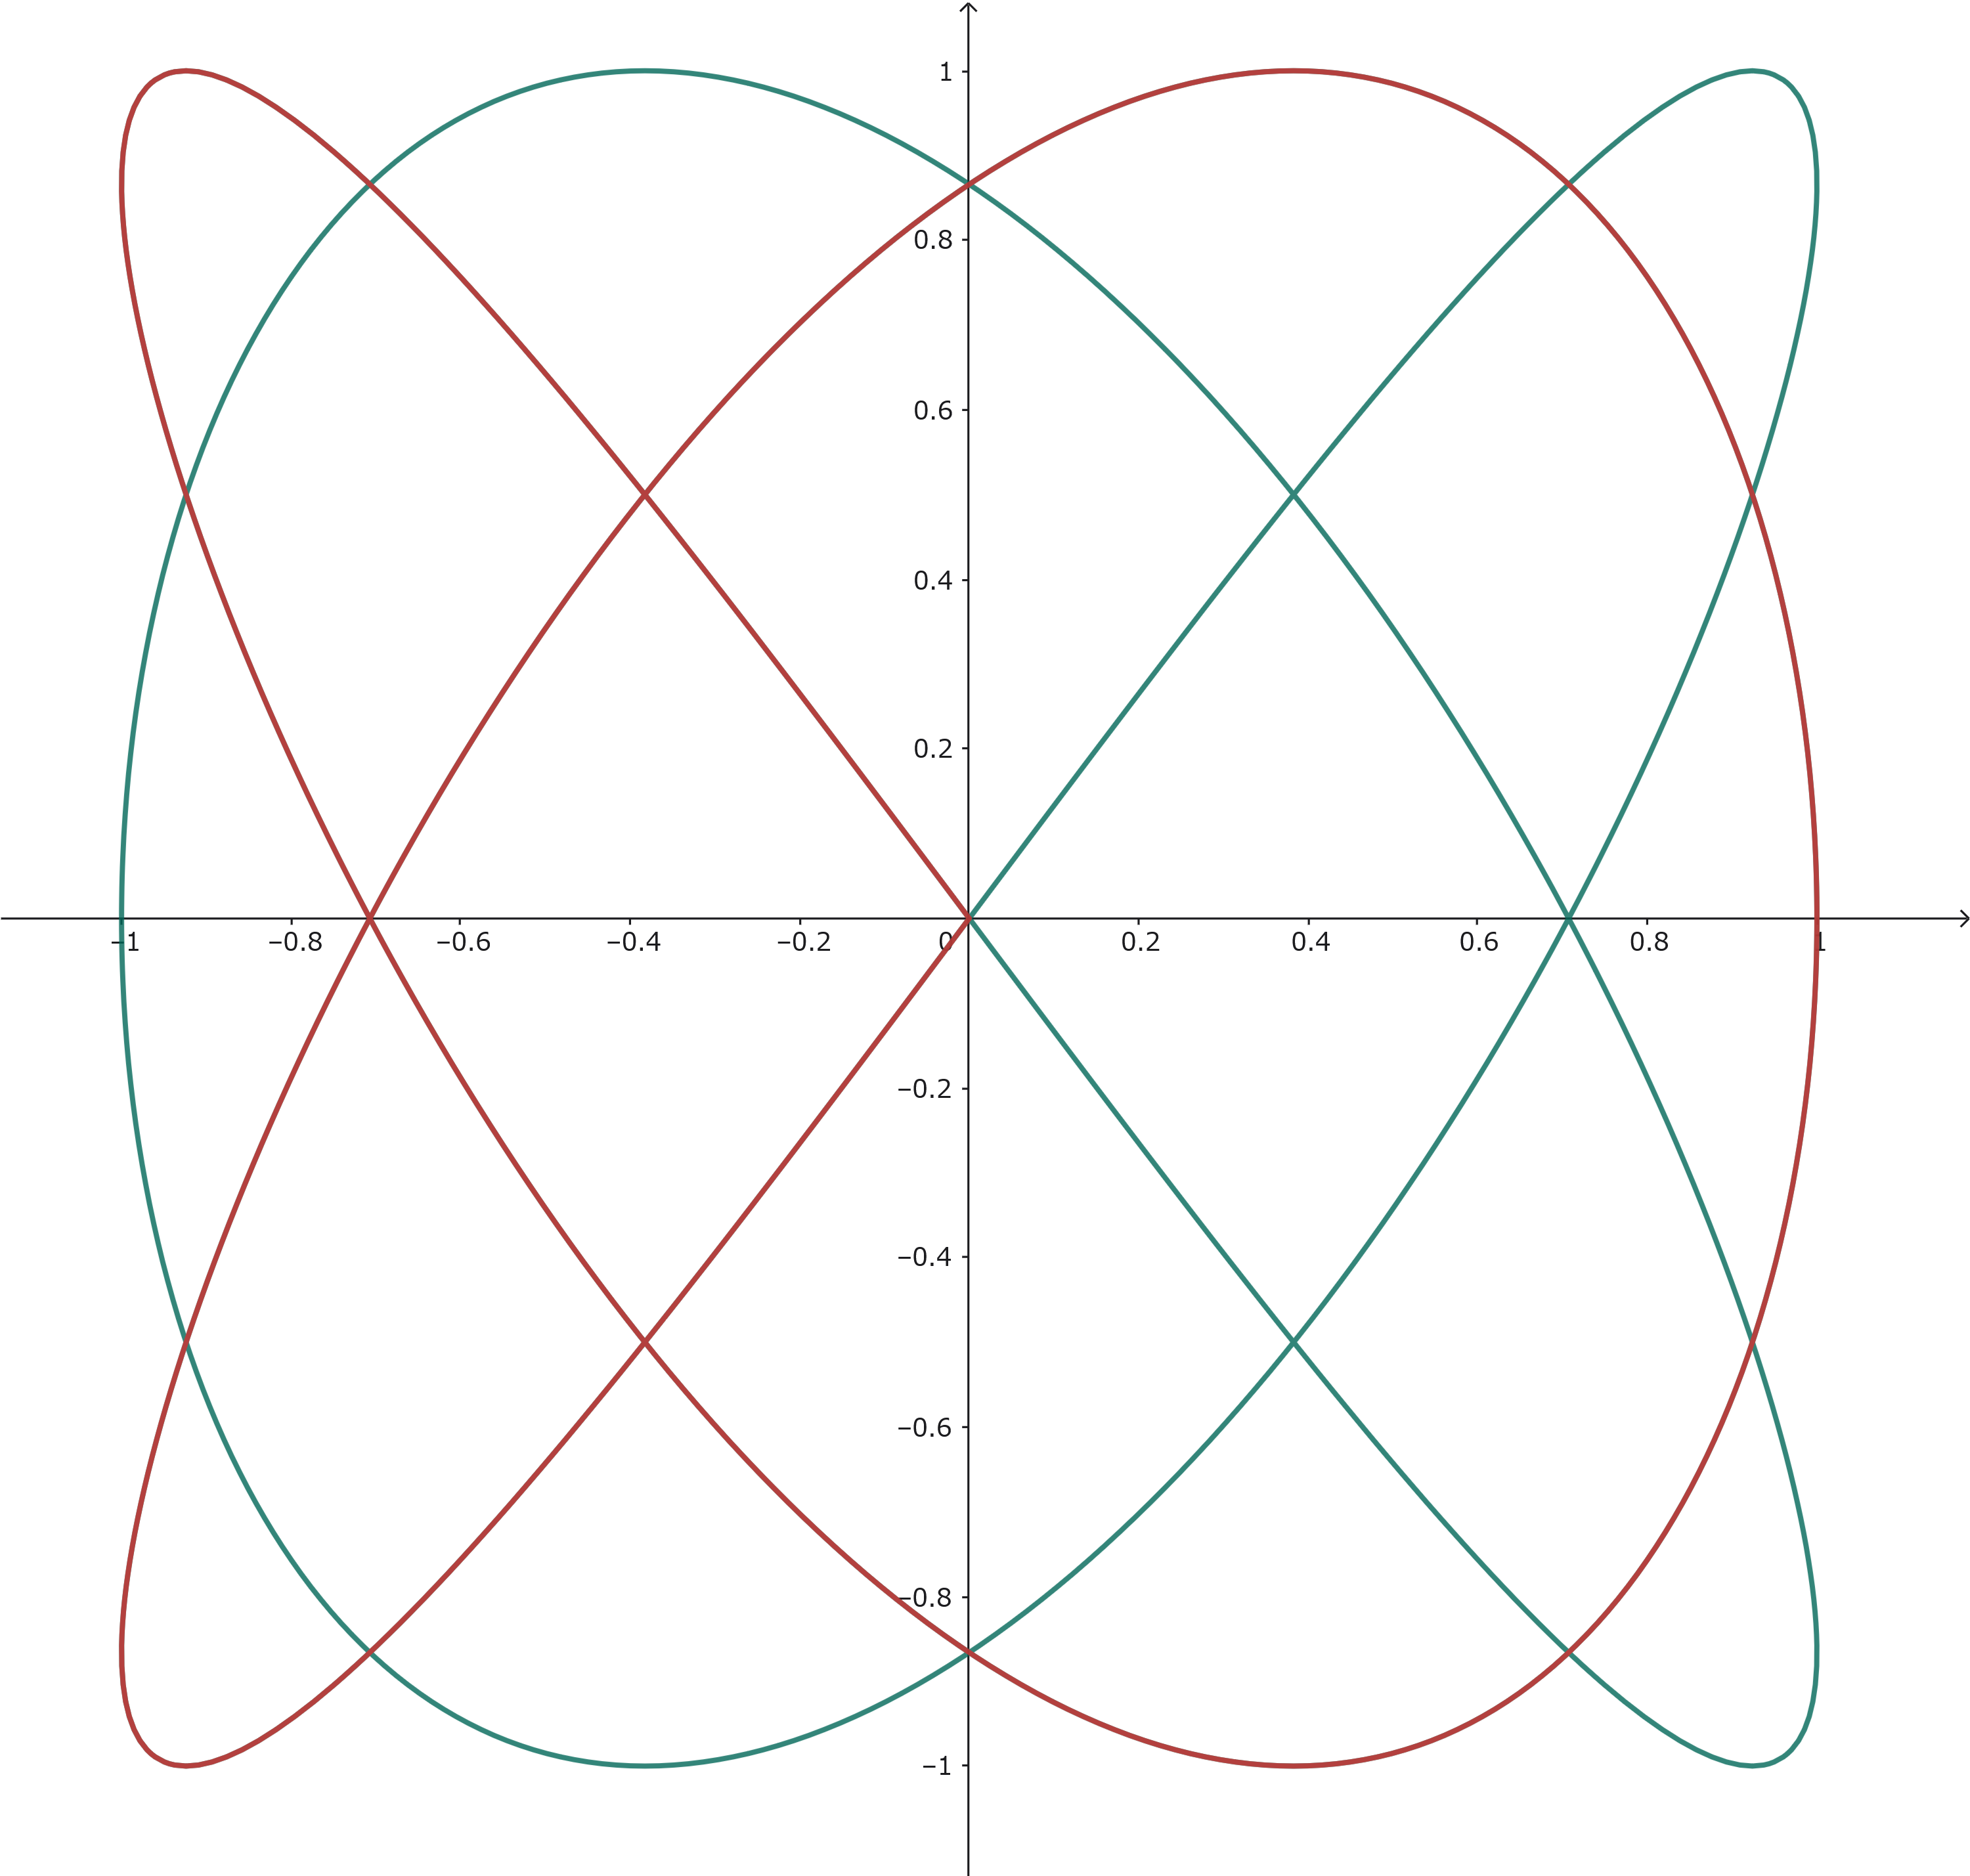
\includegraphics[scale=2.0]{img/Lissajous_curve_3_4.png}
  \caption{$m=3,n=4$。緑が$t=0\sim\pi$、赤が$t=\pi\sim2\pi$。(generated by GeoGebra)}
\end{figure}